\documentclass{report}
% PACKAGES
\usepackage{adjustbox}
\usepackage{amsmath}
\usepackage{amssymb}
\usepackage{bodegraph}
\usepackage{bbm}
\usepackage{circledsteps}
\usepackage{circuitikz}
\usepackage{enumerate}
\usepackage{mathtools}
\usepackage{nicematrix}
\usepackage{pgfplots}
\usepackage{polynom}
\usepackage{qtree}
\usepackage{rotating}
\usepackage[usestackEOL]{stackengine}
\usepackage[subpreambles=true]{standalone}
\usepackage{steinmetz}
\usepackage{subcaption}
\usepackage{tabularray}
\usepackage{tcolorbox}
\usepackage{tikz}
\usepackage{xcolor}

\usepackage[colorlinks=true,linkcolor=blue,urlcolor=black,bookmarksopen=true]{hyperref}
\usepackage{bookmark}

\usetikzlibrary{shapes.arrows}
\usetikzlibrary{shapes.misc}
\usetikzlibrary{backgrounds}
\tikzset{cross/.style={cross out, draw=black, minimum size=2*(#1-\pgflinewidth), inner sep=0pt, outer sep=0pt},
%default radius will be 1pt. 
cross/.default={1pt}}

\renewcommand{\Re}{\operatorname{Re}}
\renewcommand{\Im}{\operatorname{Im}}

\usepackage{pifont}
\newcommand{\cmark}{\text{\ding{51}}}
\newcommand{\xmark}{\text{\ding{55}}}

\newcommand{\circconv}[1]{\text{ \small\Circled{#1} }}

\newcommand{\tikzmark}[3][]{\tikz[remember picture,baseline] \node [anchor=base,#1](#2) {$#3$};}

\pgfplotsset{compat=1.18}
\pgfplotsset{
    dirac/.style={
        mark=triangle*,
        mark options={scale=1.5},
        ycomb,
        scatter,
        visualization depends on={y/abs(y)-1 \as \sign},
        scatter/@pre marker code/.code={\scope[rotate=90*\sign,yshift=-2pt]}
    }
}

\usepackage[letterpaper, portrait, margin=1.25in]{geometry}
\usepackage[font=bf]{caption}
\hbadness = 10000
\hfuzz=2pt

\newtheorem{theorem}{Theorem}[chapter]

\tikzset{every tree node/.style={anchor=north,align=center}}
\usetikzlibrary{decorations.markings}
\usetikzlibrary{arrows}
\definecolor{darkgreen}{rgb}{0.133,0.545,0.133}
\tikzstyle{n}= [circle, fill=blue, minimum size=4pt,inner sep=0pt, outer sep=0pt]

\patchcmd{\thebibliography}{\chapter*}{\section*}{}{}
\setcounter{secnumdepth}{5}

%%%%%%%%%%% EXAMPLE ENVIRONMENT %%%%%%%%%%
\usepackage{calc}
\usepackage{tabto}
\usepackage[framemethod=tikz]{mdframed} % for colored backgrounds
\newcommand{\halmos}{} % makes a box at the end

\newlength{\framedinnerleftmargin}
\newlength{\framedinnertopmargin}
\newlength{\framedreversedinnerleftmargin}
\setlength{\framedinnerleftmargin}{\widthof{Theoreme 10.10.10}+2em}
\setlength{\framedreversedinnerleftmargin}{\widthof{Theoreme 10.10.10}+1em}
\setlength{\framedinnertopmargin}{1em}
 
% first argument: label in upper left corner,
% second argument: background color
\newenvironment{boxedtext}[2]{\begin{mdframed}[%
hidealllines=true,%
backgroundcolor=#2,%
innertopmargin=\framedinnertopmargin,%
innerleftmargin=\framedinnerleftmargin,%
innerrightmargin=1em%
]%
\tabto{-\framedreversedinnerleftmargin}\textbf{#1}\tabto*{0em}%
}% begin code
{\hskip 0pt\\\hspace*{\fill}\halmos{}\end{mdframed}\vspace{1em}} % end code
 
\newenvironment{summary}[0]{\begin{center}\begin{minipage}[c]{\summarywidth}\begin{spacing}{0.9}\footnotesize} % begin code
{\end{spacing}\end{minipage}\end{center}} % end code

\newcounter{example}
 
% optional! if you want it to start at zero
% with every new chapter/section/etc.
\numberwithin{example}{section}
 
\newenvironment{example}[0]
{\refstepcounter{example}\vspace{1em plus 1em}\begin{boxedtext}{Example \theexample.}{blue!7}}%\setlength{\parskip}{0em}}
{\end{boxedtext}\vspace{-1em plus 1em}}
 
\newenvironment{example*}[0]
{\vspace{1em plus 1em}\begin{boxedtext}{Example.}{blue!7}}
{\end{boxedtext}\vspace{-1em plus 1em}}

\newmdenv[
  topline=false,
  bottomline=false,
  rightline=false,
  skipabove=\topsep,
  skipbelow=\topsep,
  linecolor=purple,
  frametitle={\noindent\textcolor{purple}{\textbf{SOLUTION }}},
  endinnercode={$\hfill\textcolor{purple}{\blacksquare}$}
]{solution}

%%%%%%%%%%%%%% COLOR BOXED %%%%%%%%%%%%%%%
% Syntax: \colorboxed[<color model>]{<color specification>}{<math formula>}
\newcommand*{\colorboxed}{}
\def\colorboxed#1#{%
  \colorboxedAux{#1}%
}
\newcommand*{\colorboxedAux}[3]{%
  % #1: optional argument for color model
  % #2: color specification
  % #3: formula
  \begingroup
    \colorlet{cb@saved}{.}%
    \color#1{#2}%
    \boxed{%
      \color{cb@saved}%
      #3%
    }%
  \endgroup
}
%%%%%%%%%%%%%%%%%%%%%%%%%%%%%%%%%%%%%%%%%

\begin{document}
\setcounter{chapter}{6}
\setcounter{page}{72}
\chapter{Discrete Fourier Transform}

We finally reach to a Fourier analysis technique that has no CT counterpart and is exclusive to DT signal processing: the discrete Fourier transform (DFT).
While there are similarities to other DT Fourier analysis techniques like the DTFT and the DTFS, the DFT is different in the sense that that the transform maps any discrete-time sequence 
to a discrete-frequency sequence. 
\begin{figure}[!hbt]
    \caption{DT Fourier analysis techniques.}
    \begin{center}
        \begin{tikzpicture}
            \node [draw,
                minimum width=2cm, 
                minimum height=1.2cm
            ] (b1) at (0,0){\Centerstack{Discrete-time\\sequence, $x[n]$}};
            \node [draw,
                minimum width=2cm, 
                minimum height=1.2cm
            ] (b2) at (3,0){DTFT};
            \node [draw,
                minimum width=2cm, 
                minimum height=1.2cm
            ] (b3) at (6,0){\Centerstack{Continuous-freq.\\function, $X(e^{j\Omega})$}};
            \draw [-latex, line width=1.5pt] (b1) -- (b2);
            \draw [-latex, line width=1.5pt] (b2) -- (b3);
        \end{tikzpicture}
    \end{center}
    \begin{center}
        \begin{tikzpicture}
            \node [draw,
                minimum width=2cm, 
                minimum height=1.2cm
            ] (b1) at (0,0){\Centerstack{Periodic\\discrete-time\\sequence, $x[n]$}};
            \node [draw,
                minimum width=2cm, 
                minimum height=1.2cm
            ] (b2) at (3,0){DTFS};
            \node [draw,
                minimum width=2cm, 
                minimum height=1.2cm
            ] (b3) at (6,0){\Centerstack{Discrete Fourier\\coefficients, $x_k$}};
            \draw [-latex, line width=1.5pt] (b1) -- (b2);
            \draw [-latex, line width=1.5pt] (b2) -- (b3);
        \end{tikzpicture}
    \end{center}
    \begin{center}
        \begin{tikzpicture}
            \node [draw,
                minimum width=2cm, 
                minimum height=1.2cm
            ] (b1) at (0,0){\Centerstack{Discrete-time\\sequence, $x[n]$}};
            \node [draw,
                minimum width=2cm, 
                minimum height=1.2cm
            ] (b2) at (3,0){DFT};
            \node [draw,
                minimum width=2cm, 
                minimum height=1.2cm
            ] (b3) at (6,0){\Centerstack{Discrete-freq.\\sequence, $X[k]$}};
            \draw [-latex, line width=1.5pt] (b1) -- (b2);
            \draw [-latex, line width=1.5pt] (b2) -- (b3);
        \end{tikzpicture}
    \end{center}
\end{figure}
\\ \\
Just as the DTFT and the DTFS are periodic, the DFT is also periodic. This makes the DFT practical for real-time use as it can be computed over a single period 
with finite resources due to its discrete-frequency nature. Additionally, relationships between different transforms make it easy for offline analyis to convert from 
the DFT spectrum to another Fourier analysis spectrum.
\\ \\
As such, the DFT is one of the most eessential tools in DSP and provides the first foray into what practicing DSP looks like.

\section{Discrete Fourier Transform}
\begin{tcolorbox}[width=\textwidth,colback={white}, sharp corners]
    The \emph{discrete Fourier transform} (DFT) of a DT signal $x[n]$ is an $N$-periodic discrete function of $k$ defined as 
    \begin{align}
        X[k] = \text{DFT}[x[n]] &= \sum_{n=0}^{N-1} x[n] e^{-j2\pi kn/N} \\
        &= \sum_{n=0}^{N-1} x[n] W^{kn}_N, \text{ for } k=0,1,...,N-1,
    \end{align}
    where $W_N=\exp(-j2\pi/N)$ is the \emph{twiddle factor}, defined for ease of notation.
\end{tcolorbox}
The DFT is essentially an operator that maps a signal defined in the \emph{continuous-time domain} to another signal defined 
in the \emph{discrete-frequency domain}. $x[n]$ and $X[k]$ constitute a unique \emph{DFT pair}. This relationship can be written as 
\begin{align}
    x[n] \iff X[k].
\end{align}
Because of this relationship, there exists an \emph{inverse DFT} defined by
\begin{align}
    x[n] = \text{DFT}^{-1}[X[k]] &= \frac{1}{N}\sum_{k=0}^{N-1} X[k] e^{+j2\pi kn/N} \\
    &= \frac{1}{N}\sum_{k=0}^{N-1} X[k] W^{-kn}_N, \text{ for } n=0,1,...,N-1.
\end{align}
Because the DFT requires both input $x[n]$ and output $X[k]$ to be discrete sequences, the DFT over a single period $N$ can be expressed as a matrix equation:
\begin{align}
    \begin{bmatrix}
        X[0] \\
        X[1] \\
        X[2] \\
        \vdots \\
        X[N-1]
    \end{bmatrix} = 
    \begin{bmatrix}
        1 & 1 & 1 & \cdots & 1 \\
        1 & W_N^1 & W_N^2 & \cdots & W_N^{(N-1)} \\
        1 & W_N^2 & W_N^4 & \cdots & W_N^{2(N-1)} \\
        \vdots & \vdots & \vdots & \ddots & \vdots \\
        1 & W_N^{(N-1)} & W_N^{2(N-1)} & \cdots & W_N^{(N-1)(N-1)}
    \end{bmatrix}
    \begin{bmatrix}
        x[0] \\
        x[1] \\
        x[2] \\
        \vdots \\
        x[N-1]
    \end{bmatrix}
\end{align}
The \emph{orthogonality principle} may be of particular use when computing the DFT by hand and is defined as 
\begin{align}
    \sum_{n=0}^{N-1} X[k] e^{j2\pi (m-k)n/N} = \left\{
    \begin{matrix}
        N, & k = m \\
        0, & k\neq m
    \end{matrix} \right\} = N\cdot\delta[k-m].
\end{align}
Note that both $x[n]$ and $X[k]$ are defined over a single period $N$. It makes sense that the transform 
is periodic, but this also means there are some implications about $x[n]$.

\begin{tcolorbox}[width=\textwidth,colback={white}, sharp corners]
    \begin{enumerate}
        \item If the DT signal is $N_0$-periodic, then by letting $N=N_0$, the DFT is simply just a scaled version of the DTFS with $X[k]=N_0 x_k$.
        \item Else if the signal is nonperiodic, then the DFT extracts the windowed signal of interest (essentially clipping a signal to finite duration of length $N$), assumes that 
        windowed signal is $N$-periodic, and essentially converts the DTFT into a DTFS with $X[k]=N x_k$.
    \end{enumerate}
\end{tcolorbox}

\pagebreak
For now, let $x[n]$ be the length-$N$ extracted DT signal. Later, we will look more into how to window a DT signal, for which $x_W[n]$ may be a more appropriate notation for the extracted signal.
\\ \\
Lastly, since the DFT is $N$-periodic, the modulo operation will be applied to the indices to represent its periodic nature. Angle brackets will be used for shorthand such that 
\begin{align}
    \langle k\rangle_N = (k \mod N).
\end{align}
When isolated to just one period for $k\in[0,N-1]$, two index equations arise: 
\begin{align}
    \langle k\rangle_N &= k, \\
    \langle -k\rangle_N &= N-k.
\end{align}
Of course, this suggests that operations related to the DFT will be cyclic in a sense. Table \ref{dft_prop} lists the properties of the DFT.
\begin{table}[!hbt]
    \centering
    \caption{Properties of the length--N DFT.}
    \label{dft_prop}
    \begin{tabular}{|c|c|c|}
        \hline
        Property & $x[n]$ & $X[k]=\text{DFT}[x[n]]$ \\[0.15cm]
        \hline
        & & \\
        Superposition & $A_1x_1[n]+A_2x_2[n]$ & $A_1X_1[k]+A_2X_2[k]$ \\[0.5cm]
        (Circular) time shift & $x[\langle n-n_0\rangle_N]$ & $e^{-j2\pi kn_0/N}X[k]=W^{kn_0}_N X[k]$ \\[0.5cm]
        Time reversal & $x[\langle -n\rangle_N]$ & $X[\langle -k\rangle_N]$ \\[0.5cm]
        Conjugation & $x^*[n]$ & $X^*[\langle -k\rangle_N]$ \\[0.5cm]
        Frequency shift & $e^{+j2\pi k_0n/N}x[n]=W^{-k_0n}_N x[n]$ & $X[\langle k-k_0\rangle_N]$ \\[0.5cm]
        Circular convolution & $x_1[n]\circledast x_2[n]$ & $X_1[k]X_2[k]$ \\[0.5cm]
        Multiplication & $x_1[n]x_2[n]$ & $\dfrac{1}{2}\left[X_1[k]\circledast X_2[k]\right]$ \\[0.5cm]
        Duality & $X[n]$ & $N\,x[\langle -k\rangle_N]$ \\[0.5cm]
        Conjugate symmetry & $x[n]$ real & 
        $\begin{cases}
            X^*[k] = X^*[\langle -k\rangle_N] \\
            \Re(X[k]) = \Re(X[\langle -k\rangle_N]) \\
            \Im(X[k]) = -\Im(X[\langle -k\rangle_N]) \\
            |X[k]| = |X[\langle -k\rangle_N]| \\
            \arg[X[k]] = -\arg[X[\langle -k\rangle_N]]
        \end{cases}$ \\[0.5cm]
         & & \\[0.25cm]
        \Centerstack{Even-odd decomposition \\ of real signals} & 
        $\begin{cases}
            x_e[n]=\frac{1}{2}[x[n]+x[\langle -n\rangle_N]] \\
            x_o[n]=\frac{1}{2}[x[n]-x[\langle -n\rangle_N]]
        \end{cases}$ & 
        $\begin{cases}
            \Re(X[k]) \\
            j\Im(X[k])
        \end{cases}$ \\[0.5cm]
        \hline
    \end{tabular}
\end{table}

\pagebreak
From the conjugate symmetry property, there are important implications about the properties of $x[n]$ and its DFT $X[k]$:
\begin{center}
    \begin{tabular}{|c|c|}
        \hline
        $x[n]$ & $X[k]$ \\
        \hline
        Real and even & Real and even \\
        Real and odd & Imaginary and odd \\
        Imaginary and even & Imaginary and even \\
        Imaginary and odd & Real and odd \\
        \hline
    \end{tabular}
\end{center}

\section{Parseval's Theorem for DFT}
Parseval's theorem for the DFT is essentially a ``conservation of (average) power'' theorem, since $x[n]$ is operated on as if periodic. When mapped from the discrete-time 
to the discrete-frequency domain, the total signal average power is conserved. It follows that the total average power of a length-$N$ DT signal $x[n]$ can be evaluated as: 
\begin{align}
    P_x = \frac{1}{N}\sum_{n=0}^{N-1} |x[n]|^2 = \sum_{k=0}^{N-1} |X[k]|^2.
\end{align}
Additionally, we can define the \emph{one-sided power spectral density} (1-sided PSD) to be 
\begin{align}
    PSD_1 = 
    \begin{cases}
        |X[0]|^2, & k=0 \\
        2|X[k]|^2, & k>0
    \end{cases}
\end{align}
and the \emph{two-sided power spectral density} (2-sided PSD) to be 
\begin{align}
    PSD_2 = |X[k]|^2.
\end{align}
Note that the 2-sided PSD is defined for all frequencies, whereas the 1-sided PSD is defined for only nonnegative frequencies. 
Because of this, the AC component of the 2-sided PSD are half the values of the 1-sided PSD. In signal processing, we tend to be more interested in the 1-sided PSD.

\section{Circular Convolution}
Here, we finally introduce the concept of \emph{circular convolution} (also called \emph{cyclic convolution} or \emph{periodic convolution}), which is different from linear convolution. 
In its simplest form, circular convolution is an operation ($\circledast$) defined by the \emph{circular convolution sum}
\begin{align}
    x[n] \circledast h[n] = \sum_{m=0}^{N-1}x[m]h[\langle n-m\rangle_N],
\end{align}
where $x[n]$ and $h[n]$ are both length-$N$. However, circular convolution also allows for convolving sequences of different lengths $N_x$ and $N_h$. For the generalized case, the symbol $\circconv{N}$ 
is used such that 
\begin{align}
    x[n] \circconv{N} h[n] = \sum_{m=0}^{N-1}x[m]h[\langle n-m\rangle_N], \text{ for } N = \max\left\{N_x,N_h\right\}.
\end{align}
Of course, this also implies that the selection of $N$ is very flexible and does not have to be the maximum length of the two sequences. Those cases will not be covered here.
\\ \\
In general, circular convolution is a temporally aliased version of the linear convolution in the time domain. As a result, we can leverage that fact by aliasing the linear convolution 
to compute the circular convolution.
\\ \\
Recall that the linear convolution of two finite sequences is given by
\begin{align}
    y_L[n] = x[n] * h[n] = \sum_{m=-\infty}^{+\infty}x[m]h[n-m],
\end{align}
with $(\text{domain }x[n])=[0,N_x-1]$ and $(\text{domain }h[n])=[0,N_h-1]$. Then by wrapping the linear convolution sequence, the circular convolution over one period $n\in[0,N-1]$ for $N=\max\left\{N_x,N_h\right\}$ can be defined as 
\begin{align}
    x[n] \circconv{N} h[n] = 
    \begin{cases}
        y_L[n] + y_L[n+N], & 0 \leq n < N_L-N \\
        y_L[n], & \text{otherwise}.
    \end{cases}
\end{align}

\begin{example}
    Use temporal aliasing to find $y[n]=x[n]\circledast h[n]$, given that 
    \begin{align*}
        x[n] &= \left\{\underbar{2},1,4,3\right\}, \\
        h[n] &= \left\{\underbar{5},3,2,1\right\}.
    \end{align*}
\end{example}
\begin{solution}
    Note that the period for both sequences is $N=4$. Setting up the condensed tabular method for linear convolution: 
    \begin{center}
        \begin{NiceTabular}{p{1cm}|p{1cm} p{1cm} p{1cm} p{1cm}}[corners=NE,margin]
            \rule{0pt}{2em}\diagbox{$x[n]$}{$h[n]$} & \Block{1-1}{$\underline{5}$} & \Block{1-1}{3} & \Block{1-1}{2} & \Block{1-1}{1} \\
            \hline
            \Block{1-1}{$\underline{2}$} & \Block[fill=yellow!50]{1-1}{10} & \Block[fill=red!30]{1-1}{6} & \Block[fill=blue!30]{1-1}{4} & \Block[fill=green!30]{1-1}{2} \\
            \Block{1-1}{1} & \Block[fill=red!30]{1-1}{5} & \Block[fill=blue!30]{1-1}{3} & \Block[fill=green!30]{1-1}{2} & \Block[fill=violet!30]{1-1}{1} \\
            \Block{1-1}{4} & \Block[fill=blue!30]{1-1}{20} & \Block[fill=green!30]{1-1}{12} & \Block[fill=violet!30]{1-1}{8} & \Block[fill=orange!50]{1-1}{4} \\
            \Block{1-1}{3} & \Block[fill=green!30]{1-1}{15} & \Block[fill=violet!30]{1-1}{9} & \Block[fill=orange!50]{1-1}{6} & \Block[fill=cyan!30]{1-1}{3}
        \end{NiceTabular}
    \end{center}
    Each right-to-left diagonal is highlighted a different color to show which entries should be summed. Then the linear convolution is given by:
    \begin{align*}
        y_L[n] &= \left\{\underbar{10},6+5,4+3+20,2+2+12+15,1+8+9,4+6,3\right\} \\
        &= \left\{\underbar{10},11,27,31,18,10,3\right\}.
    \end{align*}
    Then by aliasing the output, the circular convolution is given by:
    \begin{align*}
        x[n] \circledast h[n] &= 
        \begin{cases}
            y_L[n] + y_L[n+4], & 0 \leq n < (7-4) \\
            y_L[n], & \text{otherwise}
        \end{cases} \\
        &= \left\{\underbar{10+18},11+10,27+3,31\right\} \\
        &= \left\{\underbar{28},21,30,31\right\}.
    \end{align*}
\end{solution}

\begin{example}
    Use the DFT to find $y[n]=x[n]\circledast h[n]$, given that 
    \begin{align*}
        x[n] &= \left\{\underbar{2},1,4,3\right\}, \\
        h[n] &= \left\{\underbar{5},3,2,1\right\}.
    \end{align*}
\end{example}
\begin{solution}
    From the table of DFT properties, we can multiply the DFTs of the two sequences and then compute the inverse DFT of the product. Then for $N=4$:
    \begin{align*}
        X[0] &= \sum_{n=0}^{N-1} x[n] e^{-j2\pi (0)n/N} = 2 + 1 + 4 + 3 = 10 \\
        X[1] &= \sum_{n=0}^{N-1} x[n] e^{-j2\pi (1)n/N} = 2 - j1 - 4 + j3 = -2+j2 \\
        X[2] &= \sum_{n=0}^{N-1} x[n] e^{-j2\pi (2)n/N} = 2 - 1 + 4 - 3 = 2 \\
        X[3] &= \sum_{n=0}^{N-1} x[n] e^{-j2\pi (3)n/N} = 2 + j1 - 4 - j3 = -2-j2 \\
        & \cdots \\
        H[0] &= \sum_{n=0}^{N-1} h[n] e^{-j2\pi (0)n/N} = 5 + 3 + 2 + 1 = 11 \\
        H[1] &= \sum_{n=0}^{N-1} h[n] e^{-j2\pi (1)n/N} = 5 - j3 - 2 + j1 = 3-j2 \\
        H[2] &= \sum_{n=0}^{N-1} h[n] e^{-j2\pi (2)n/N} = 5 - 3 + 2 - 1 = 3 \\
        H[3] &= \sum_{n=0}^{N-1} h[n] e^{-j2\pi (3)n/N} = 5 + j3 - 2 - 1 = 3+j2
    \end{align*}
    Performing pointwise multiplication, we get 
    \begin{align*}
        Y[0] &= X[0]H[0] = (10)(11) = 110 \\
        Y[1] &= X[1]H[1] = (-2+j2)(3-j2) = -2+j10 \\
        Y[2] &= X[2]H[2] = (2)(3) = 6 \\
        Y[3] &= X[3]H[3] = (-2-j2)(3+j2) = -2-j10
    \end{align*}
    Lastly, compute the inverse DFT.
    \begin{align*}
        y[0] &= \frac{1}{N}\sum_{k=0}^{N-1} Y[k] e^{+j2\pi k(0)/N} = \frac{1}{4}[110 + (-2+j10) + 6 + (-2-j10)] = 28 \\
        y[1] &= \frac{1}{N}\sum_{k=0}^{N-1} Y[k] e^{+j2\pi k(1)/N} = \frac{1}{4}[110 + j(-2+j10) - 6 - j(-2-j10)] = 21 \\
        y[2] &= \frac{1}{N}\sum_{k=0}^{N-1} Y[k] e^{+j2\pi k(2)/N} = \frac{1}{4}[110 - (-2+j10) + 6 - (-2-j10)] = 30 \\
        y[3] &= \frac{1}{N}\sum_{k=0}^{N-1} Y[k] e^{+j2\pi k(3)/N} = \frac{1}{4}[110 - j(-2+j10) - 6 + j(-2-j10)] = 31
    \end{align*}
    Though tedious, we get the same solution as the aliasing method.
\end{solution}

While circular convolution is not the same as linear convolution, \emph{zero-padding} can be used with circular convolution to obtain 
the same output as linear convolution. Let 
\begin{align}
    z_x[n] &= \{\underbar{\emph{x}[0]},x[1],...,x[N_x-1], \underbrace{0,0,...,0}_{N-N_x}\}, \\
    z_h[n] &= \{\underbar{\emph{h}[0]},h[1],...,h[N_h-1], \underbrace{0,0,...,0}_{N-N_h}\}, \text{ for } N\geq N_x+N_h-1.
\end{align}
Then the unaliased linear convolution can be retrieved from the circular convolution of two zero-padded sequences:
\begin{align}
    y_L[n] &= z_x[n] \circconv{N} z_h[n], \text{ for } N\geq N_x+N_h-1.
\end{align}

\section{Relationships Between Transforms}
It can be said that the DFT is a sampled version of the DTFT, with 
\begin{align}
    X[k] = X(e^{j\Omega})\big|_{\Omega=2\pi k/N}.
\end{align}
By virtue of the $z$--transform being related to the DTFT, it can also be said that the DFT samples the unit circle of the $z$--transform such that 
\begin{align}
    X[k] = X(z)\big|_{z=\exp(j2\pi k/N)}.
\end{align}
Figure \ref{flowchart} shows the relationships between all CT and DT transforms that we have learned so far. As such, 
this marks the end of theory-based signals and systems as we begin moving towards DSP in practice.

\begin{figure}
    \caption{Relationships between transforms.}
    \label{flowchart}
    \centering
    \includestandalone[mode=buildnew, width=\textwidth]{flowchart}
\end{figure}

\section{Recontextualizing the DFT}
From what we already know, when extracting a length-$N$ data sequence $x[n]$ and taking the DFT, we get some length-$N$ 
sampled frequency spectrum $X[k]$. Now let us introduce some new terminology and variables that are more common in practice.

\subsection{Time-Domain Terminology}
From before, the \emph{sampling rate} is the number of samples taken per second from a CT signal to create a DT signal and is defined as 
\begin{align}
    f_s = \frac{1}{T_s} \text{ [samp/sec]},
\end{align}
where $T_s$ is the sampling period (or sampling interval), or the amount of time between consecutive samples. This extracted sequence $x[n]$ is typically causal and is referred to as a \emph{frame} of data. 
\\ \\
We also now redefine the sampling period as \emph{temporal resolution}, 
which is a measurement of how fine the spacing between the time samples are and is defined as 
\begin{align}
    \Delta t = T_s = \frac{1}{f_s} \text{ [sec]}.
\end{align}
The point $x[n_0]$ is referred to as the \emph{time sample} at time index $n_0$. 
The actual \emph{elapsed time} at $n_0$ is given by $n_0\Delta t$.
\\ \\
Instead of referring to $x[n]$ as length-$N$, we say that the \emph{frame size} or (\emph{frame length}) is $N$: 
\begin{align}
    N = \text{count}(x[n])  \text{ [samp]}.
\end{align}
The \emph{frame time} is the total amount of time corresponding to frame size $N$ and is given by 
\begin{align}
    T_f = N\Delta t = \frac{N}{f_s}  \text{ [sec]}.
\end{align}
Its reciprocal is referred to as the \emph{frame rate} of the signal.

\begin{figure}[!hbt]
    \centering
    \caption{Frame of data in the time domain.}
    \begin{tikzpicture}
        [declare function={
            func(\x)= 2.5 + 1.5*cos(deg(\x)) ; }]
        \begin{axis}[
            axis x line=center, axis y line=center,
            ymin=-2, ymax=6, ytick={0}, 
            xmin=-0.5, xmax=8, xtick={0},
            domain=0:7.5, samples=100,
            extra x ticks={0}, extra x tick labels={\scriptsize\Centerstack{ \\ }}, 
            width=12cm, height=7cm]
            \addplot+ [
                ycomb, 
                domain=0:6, 
                samples=10,
            ] {func(x)};
            \addlegendentry{$x[n]$}
            \addplot [red,thick]{func(x)};
            \addlegendentry{$x(t)$}
            \draw[latex-latex] (6/9,-0.4) to node[midway,below] {$\Delta t=1/f_s$} (12/9,-0.4);
            \draw[latex-latex, darkgreen] (0/9,-1.25) to node[midway,below] {$T_f=N\Delta t$} (10*6/9-0.2,-1.25);
            \node[] at (3.45,5.1) {$N$};
            \draw[-latex,orange] (3.2,5) to (0*6/9+0.1,{func(0*6/9)+0.1});
            \draw[-latex,orange] (3.25,4.9) to (1*6/9+0.1,{func(1*6/9)+0.1});
            \draw[-latex,orange] (3.3,4.8) to (2*6/9+0.1,{func(2*6/9)+0.1});
            \draw[-latex,orange] (3.35,4.7) to (3*6/9+0.05,{func(3*6/9)+0.1});
            \draw[-latex,orange] (3.4,4.6) to (4*6/9+0.05,{func(4*6/9)+0.1});
            \draw[-latex,orange] (3.45,4.5) to (5*6/9+0,{func(5*6/9)+0.1});
            \draw[-latex,orange] (3.5,4.6) to (6*6/9-0.05,{func(6*6/9)+0.1});
            \draw[-latex,orange] (3.55,4.7) to (7*6/9-0.05,{func(7*6/9)+0.1});
            \draw[-latex,orange] (3.6,4.8) to (8*6/9-0.1,{func(8*6/9)+0.1});
            \draw[-latex,orange] (3.65,4.9) to (9*6/9-0.1,{func(9*6/9)+0.1});
        \end{axis}
    \end{tikzpicture}
\end{figure}

\subsection{Frequency-Domain Terminology}
From before, the sampling rate $f_s$ should follow the Nyquist--Shannon sampling theorem such that 
a CT signal with highest frequency content at $f_{max}$ can be captured under the criterion
\begin{align}
    f_s \geq \frac{f_{max}}{2} \text{ [samp/sec]},
\end{align}
with the Nyquist frequency defined at equality. 
This highest frequency $f_{max}$ is referred to as the \emph{bandwidth} of the signal being sampled.
\\ \\
As mentioned before, when performing the DFT, the transform essentially samples the DTFT spectrum. Because 
the frame size is $N$, we would take the length-$N$ DFT. In other words, the \emph{DFT size} is $N$. 
Just as the frame is defined by frame size $N$, the DFT spectrum is defined by DFT size $N$.
\\ \\
The \emph{frequency resolution} then is a measurement of how fine the spacing between the spectral samples are 
and is defined as 
\begin{align}
    \Delta f = \frac{f_s}{N} \text{ [Hz]}.
\end{align}
The point $X[k_0]$ is referred to as the \emph{spectral sample} at frequency index $k_0$. The spacing between frequency indices 
$k_m$ and $k_{m+1}$ is called the $m^{th}$ \emph{frequency bin}.
\\ \\
The \emph{frequency range} of the (two-sided) spectrum corresponding to DFT size $N$ is given by 
\begin{align}
    F = N\Delta f \text{ [Hz]}.
\end{align}

\begin{figure}[!hbt]
    \centering
    \caption{DFT spectrum in the frequency domain.}
    \label{dft_spec}
    \begin{tikzpicture}
        [declare function={
            func(\x)= and(\x > -2, \x < 2) * 3*(1-abs(\x/2)) ; }]
        \begin{axis}[
            axis x line=center, axis y line=center,
            ymin=-2, ymax=5, ytick={0}, 
            xmin=-0.5, xmax=8, xtick={0},
            domain=0:7.5, samples=100,
            extra x ticks={0}, extra x tick labels={\scriptsize\Centerstack{ \\ }}, 
            width=12cm, height=7cm]
            \addplot+ [
                ycomb, 
                domain=0:(6*9/10), 
                samples=11,
            ] {func(x)+func(x-6)};
            \addlegendentry{$X[k]$}
            \addplot [red,thick]{func(x)+func(x-6)};
            \addlegendentry{$X(e^{j2\pi r})$}
            \draw[latex-latex] (6/11,-0.4) to node[midway,below] {$\Delta f=f_s/N$} (12/11,-0.4);
            \draw[latex-latex, darkgreen] (0/9,-1.25) to node[midway,below] {$F=N\Delta f$} (6*9/10+0.4,-1.25);
            \node[] at (3.45,4.1) {$N$};
            \draw[-latex,orange] (3.2,4) to (0*6/11+0.1,{func(0*6/11)+0.1});
            \draw[-latex,orange] (3.25,3.9) to (1*6/11+0.1,{func(1*6/11)+0.1});
            \draw[-latex,orange] (3.3,3.8) to (2*6/11+0.1,{func(2*6/11)+0.1});
            \draw[-latex,orange] (3.35,3.7) to (3*6/11+0.05,{func(3*6/11)+0.1});
            \draw[-latex,orange] (3.4,3.6) to (4*6/11+0.05,{func(4*6/11)+0.1});
            \draw[-latex,orange] (3.45,3.5) to (5*6/11+0,{func(5*6/11)+0.1});
            \draw[-latex,orange] (3.5,3.6) to (6*6/11-0.05,{func(5*6/11)+0.1});
            \draw[-latex,orange] (3.55,3.7) to (7*6/11-0.05,{func(4*6/11)+0.1});
            \draw[-latex,orange] (3.6,3.8) to (8*6/11-0.1,{func(3*6/11)+0.1});
            \draw[-latex,orange] (3.65,3.9) to (9*6/11-0.1,{func(2*6/11)+0.1});
            \draw[-latex,orange] (3.7,4) to (10*6/11-0.1,{func(1*6/11)+0.1});
        \end{axis}
    \end{tikzpicture}
\end{figure}
While not presented as two-sided, typically the latter half of the spectrum is shifted one period to the left to form 
a more meaningful sampled spectrum, as seen going from Fig. \ref{dft_spec} to Fig. \ref{dft_spec_shift}. Going forward, we will 
assume the circularly shifted form of the spectrum.
\\ \\
Lastly, while not as common, \emph{angular frequency resolution} can be defined as 
\begin{align}
    \Delta \omega = \frac{2\pi f_s}{N} = 2\pi\Delta f.
\end{align}
This relationship becomes important if one were to choose to plot the spectrum in terms of angular frequency.
\begin{figure}[!hbt]
    \centering
    \caption{Circularly shifted DFT spectrum in the frequency domain.}
    \label{dft_spec_shift}
    \begin{tikzpicture}
        [declare function={
            func(\x)= and(\x > -2, \x < 2) * 3*(1-abs(\x/2)) ; }]
        \begin{axis}[
            axis x line=center, axis y line=center,
            ymin=-2, ymax=5, ytick={0}, 
            xmin=-4.5, xmax=4, xtick={0},
            domain=-4:4, samples=100,
            extra x ticks={0}, extra x tick labels={\scriptsize\Centerstack{ \\ }}, 
            width=12cm, height=7cm]
            \addplot+ [
                ycomb, 
                domain=-(3*9/10):(3*9/10), 
                samples=11,
            ] {func(x)};
            \addlegendentry{$X[k]$}
            \addplot [red,thick]{func(x)+func(x-6)};
            \addlegendentry{$X(e^{j2\pi r})$}
        \end{axis}
    \end{tikzpicture}
\end{figure}

\pagebreak
\section{Error Sources in the DFT}
Due to the discrete and implicitly periodic nature of the DFT, the DFT is prone to capturing some errors. This section will briefly cover the main sources and potential solutions.

\subsection{Aliasing}
As seen before in undersampled signals as well as downsampled signals, \emph{aliasing} is a type of signal distortion caused by spectral overlap between neighboring spectral copies in the frequency domain. 
Essentially, the higher frequency content unintentionally becomes amplified and more prominent in the captured signal, thus contaminating the original time signal. 
When performing the DFT on the contaminated signal, we would get a sampled version of this distorted frequency spectrum.
\begin{center}
    \begin{tikzpicture}
        [declare function={
            func(\x)= and(\x > -4, \x < 4) * (1-abs(\x/4)); }]
        \begin{axis}[
            axis x line=center, axis y line=center,
            ymin=0, ymax=1, ytick={0}, ylabel={$X(e^{j\Omega})$},
            xmin=-7.5, xmax=7.5, xtick={0},
            domain=-7:7, samples=200,
            width=8cm, height=4cm]
            \addplot [blue,thick]{func(x)/2};
            \addplot [red,thick]{func(x+2*pi)/2};
            \addplot [red,thick]{func(x-2*pi)/2};
            \node[] at (3,0.4) {\scriptsize\Centerstack{Aliasing\\$\downarrow$}};
        \end{axis}
    \end{tikzpicture} $\Longrightarrow$
    \begin{tikzpicture}
        [declare function={
            func(\x)= and(\x > -4, \x < 4) * (1-abs(\x/4)); }]
        \begin{axis}[
            axis x line=center, axis y line=center,
            ymin=0, ymax=1, ytick={0}, ylabel={$X(e^{j\Omega})$},
            xmin=-7.5, xmax=7.5, xtick={0},
            domain=-7:7, samples=200,
            width=8cm, height=4cm]
            \addplot+ [
                ycomb, 
                domain=-3.2:3.2, 
                samples=9,
            ] {func(x)/2 + func(x+2*pi)/2 + func(x-2*pi)/2};
            \addplot [red,thick]{func(x)/2 + func(x+2*pi)/2 + func(x-2*pi)/2};
            \node[] at (3,0.4) {\scriptsize\Centerstack{Aliasing\\$\downarrow$}};
        \end{axis}
    \end{tikzpicture}
\end{center}
There are two possible methods to combat (spectral) aliasing. The first possible solution is to increase the sampling rate. This is typically done at the hardware-level, in which the the DSP engineer would 
upgrade or replace the ADC containing the sampler.
\\ \\
The second possible solution is to apply an anti-aliasing filter. As seen before with decimated signals, an anti-aliasing filter essentially restrict the bandwidth of the undersampled signal to remove all undesired 
higher frequency content that is causing the distortion. The cutoff frequency is typically at half the Nyquist frequency. This however also means that the recovered signal inevitably has some information loss.
\begin{center}
    \begin{tikzpicture}
        [declare function={
            func(\x)= and(\x > -4, \x < 4) * (1-abs(\x/4)); }]
        \begin{axis}[
            axis x line=center, axis y line=center,
            ymin=0, ymax=1, ytick={0}, ylabel={$X(e^{j\Omega})$},
            xmin=-7.5, xmax=7.5, xtick={0},
            domain=-7:7, samples=200,
            width=8cm, height=4cm]
            \addplot [blue,thick]{func(x)/2};
            \addplot [red,thick]{func(x+2*pi)/2};
            \addplot [red,thick]{func(x-2*pi)/2};
            \draw[darkgreen] (-2.28,0)--(-2.28,0.7)--(2.28,0.7)--(2.28,0);
        \end{axis}
    \end{tikzpicture} $\Longrightarrow$
    \begin{tikzpicture}
        [declare function={
            func(\x)= and(\x > -2.28, \x < 2.28) * (1-abs(\x/4)); }]
        \begin{axis}[
            axis x line=center, axis y line=center,
            ymin=0, ymax=1, ytick={0}, ylabel={$X(e^{j\Omega})$},
            xmin=-7.5, xmax=7.5, xtick={0},
            domain=-7:7, samples=200,
            width=8cm, height=4cm]
            \addplot+ [
                ycomb, 
                domain=-3.2:3.2, 
                samples=9,
            ] {func(x)/2};
            \addplot [red,thick]{func(x)/2 + func(x+2*pi)/2 + func(x-2*pi)/2};
        \end{axis}
    \end{tikzpicture}
\end{center}

\subsection{Picket-Fence Effect}
The \emph{picket-fence effect} (also called \emph{scalloping loss}) is the phenomenon of missing pertinent frequency artifacts (such as 
a large spectral component or a spectral null) that occur mid-bin in the DFT spectrum due to insufficient frequency sampling. Recall that both the frame size and the DFT spectrum share 
the same value $N$; if not enough time samples are taken, that also gets reflected in the small number of spectral samples computed.
\begin{center}
    \begin{tikzpicture}
        [declare function={
            func(\x)= and(\x > -4, \x < 4) * (1-abs(\x/4)); }]
        \begin{axis}[
            axis x line=center, axis y line=center,
            ymin=0, ymax=1, ytick={0}, ylabel={$X_{\langle 2\pi\rangle}(e^{j\Omega})$},
            xmin=-7.5, xmax=7.5, xtick={0},
            domain=-4:4, samples=100,
            width=8cm, height=4cm]
            \addplot+ [
                ycomb, 
                domain=-4:4, 
                samples=6,
            ] {func(x)/2};
            \addplot [red,thick]{func(x)/2};
            \node[] at (4,0.5) {\scriptsize $\leftarrow$ Peak at mid-bin};
        \end{axis}
    \end{tikzpicture} $\Longrightarrow$
    \begin{tikzpicture}
        [declare function={
            func(\x)= and(\x > -4, \x < 4) * (1-abs(\x/4)); }]
        \begin{axis}[
            axis x line=center, axis y line=center,
            ymin=0, ymax=1, ytick={0}, ylabel={\shortstack{$X_{\langle 2\pi\rangle}(e^{j\Omega})$\\(scalloped)}},
            xmin=-7.5, xmax=7.5, xtick={0},
            domain=-7:7, samples=200,
            width=8cm, height=4cm]
            \addplot+ [
                ycomb, 
                domain=-4:4, 
                samples=6,
            ] {func(x)/2};
            \draw[thick,red] (-4,0)--(-2.4,0.2)--(-0.8,0.4)--(0.8,0.4)--(2.4,0.2)--(4,0);
        \end{axis}
    \end{tikzpicture}
\end{center}
There is a simple solution to this problem. Recall that the frequency resolution is given by $\Delta f=f_s/N$. Keeping the sampling rate the same, 
one can increase the frame size $N$ by zero-padding the original extracted sequence such that the frequency resolution gets finer, and more spectral samples are collected. 
\begin{center}
    \begin{tikzpicture}
        [declare function={
            func(\x)= and(\x > -4, \x < 4) * (1-abs(\x/4)); }]
        \begin{axis}[
            axis x line=center, axis y line=center,
            ymin=0, ymax=1, ytick={0}, ylabel={$X_{\langle 2\pi\rangle}(e^{j\Omega})$},
            xmin=-7.5, xmax=7.5, xtick={0},
            domain=-4:4, samples=100,
            width=8cm, height=4cm]
            \addplot+ [
                ycomb, 
                domain=-4:4, 
                samples=11,
            ] {func(x)/2};
            \addplot [red,thick]{func(x)/2};
        \end{axis}
    \end{tikzpicture}
\end{center}

\subsection{Windowing and Spectral Leakage}
\emph{Windowing} is the process of extracting a frame of data by multiplying the original source signal $s[n]$ by a finite-duration \emph{window function} $w[n]$. 
Mathematically, this is represented by 
\begin{align}
    x[n] = s[n]w[n],
\end{align}
where $x[n]$ is the extracted frame of data. Since the window $w[n]$ is typically a rectangular sequence, the windowed sequence is given by
\begin{align}
    x[n] = \begin{cases}
        s[n], & 0\leq n<N-1 \\
        0, & \text{otherwise}.
    \end{cases}
\end{align}
\begin{center}
    \begin{tikzpicture}
        [declare function={
            func(\x)= 1+sin(deg(\x*pi/3)); }]
        \begin{axis}[
            axis x line=center, axis y line=center,
            ymin=0, ymax=3, ytick={0}, ylabel={$s[n]$},
            xmin=-0.5, xmax=9, xtick={0},
            domain=0:8, samples=100,
            width=8cm, height=4cm]
            \addplot+ [
                ycomb, 
                domain=0:8, 
                samples=12,
            ] {func(x)};
            \addplot [red,thick]{func(x)};
            \draw[dashed,darkgreen] (-0.1,0)--(-0.1,2.3)--(5.2,2.3)--(5.2,0);
            \node[darkgreen] at (4,2) {$w[n]$};
        \end{axis}
    \end{tikzpicture} $\Longrightarrow$
    \begin{tikzpicture}
        [declare function={
            func(\x)= (1+sin(deg(\x*pi/3))) * (\x < 5.2); }]
        \begin{axis}[
            axis x line=center, axis y line=center,
            ymin=0, ymax=3, ytick={0}, ylabel={$x[n]$},
            xmin=-0.5, xmax=9, xtick={0},
            domain=0:8, samples=100,
            width=8cm, height=4cm]
            \addplot+ [
                ycomb, 
                domain=0:8, 
                samples=12,
            ] {func(x)};
            \draw[dashed,darkgreen] (-0.1,0)--(-0.1,2.3)--(5.2,2.3)--(5.2,0);
            \node[darkgreen] at (4,2) {$w[n]$};
        \end{axis}
    \end{tikzpicture}
\end{center}
Of course, this is implies that two different source signals can have the same windowed signal and thus 
the same DFT due to the DFT's assumption of periodicity.
\\ \\
Additionally, the rectangular window is an ideal window for the DFT as its DTFT is the Dirichlet kernel (also called the periodic sinc), 
which acts as a convolution filter in $\Omega$ that interpolates between frequency bins. The higher the frame size $N$, the more 
accurate the DFT is as the sampled DTFT.
\\ \\
However, because of this assumed periodicity, \emph{spectral leakage} can occur, in which the presence of endpoint discontinuities (called \emph{edge discontinuities}) can introduce 
higher-frequency distortion, forcing the DFT spectrum to redistribute its power as power undesirably ``leaks'' from large spectral components to neighboring 
frequencies (essentially a smearing effect). 
\\ \\
There are two ways endpoint discontinuities can occur. First, if the source signal is already periodic itself, then edge discontinuities can occur if the windowed sequence does not contain 
an integer number of cycles. Below shows what happens when such sampled signals are interpolated and periodically ``stitched'' to form the distorted periodic signal.
\begin{center}
    \begin{tikzpicture}
        [declare function={
            func(\x)= 1+sin(deg(\x*pi/3)); }]
        \begin{axis}[
            axis x line=center, axis y line=center,
            ymin=0, ymax=3, ytick={0}, ylabel={$s(t)$},
            xmin=-0.5, xmax=15, xtick={0},
            domain=-1:16, samples=100,
            width=8cm, height=4cm]
            \addplot [red,thick]{func(x)};
            \draw[dashed,darkgreen] (0,0)--(0,2.3)--(5,2.3)--(5,0);
            \node[darkgreen] at (4,2) {$w(\cdot)$};
        \end{axis}
    \end{tikzpicture} $\Longrightarrow$
    \begin{tikzpicture}
        [declare function={
            func(\x)= (1+sin(deg(\x*pi/3))) * and(\x>=0,\x<5); }]
        \begin{axis}[
            axis x line=center, axis y line=center,
            ymin=0, ymax=3, ytick={0}, ylabel={$x(t)$ (interpolated)},
            xmin=-0.5, xmax=15, xtick={0},
            domain=-1:16, samples=100,
            width=8cm, height=4cm]
            \addplot [red,thick]{func(x)+func(x-5)+func(x-10)+func(x+5)};
            \node[] at (4,1.5) {\scriptsize\Centerstack{Edge\\discont-\\inuity\\$\searrow$}};
        \end{axis}
    \end{tikzpicture}
\end{center}
The second and more common way assumes source signals are nonperiodic (such as speech signals). Regardless of where the windowing ends, unintentional sharp transitions between the endpoints of 
a windowed sequence introduce edge discontinuities that can cause spectral leakage.
\begin{center}
    \begin{tikzpicture}
        [declare function={
            func(\x)= 2*exp(-\x/2); }]
        \begin{axis}[
            axis x line=center, axis y line=center,
            ymin=0, ymax=3, ytick={0}, ylabel={$s(t)$},
            xmin=-0.5, xmax=15, xtick={0},
            domain=-1:16, samples=100,
            width=8cm, height=4cm]
            \addplot [red,thick]{func(x)};
            \draw[dashed,darkgreen] (0,0)--(0,2.3)--(5,2.3)--(5,0);
            \node[darkgreen] at (4,2) {$w(\cdot)$};
        \end{axis}
    \end{tikzpicture} $\Longrightarrow$
    \begin{tikzpicture}
        [declare function={
            func(\x)= (2*exp(-\x/2)) * and(\x>=0,\x<5); }]
        \begin{axis}[
            axis x line=center, axis y line=center,
            ymin=0, ymax=3, ytick={0}, ylabel={$x(t)$ (interpolated)},
            xmin=-0.5, xmax=15, xtick={0},
            domain=-1:16, samples=100,
            width=8cm, height=4cm]
            \addplot [red,thick]{func(x)+func(x-5)+func(x-10)+func(x+5)};
            \node[] at (3.5,1.5) {\scriptsize\Centerstack{Edge\\discont-\\inuity\\$\searrow$}};
        \end{axis}
    \end{tikzpicture}
\end{center}
For periodic signals, one way to mitigate spectral leakage is to increase the frame size by extending the duration of the window, 
ideally until there is minimal separation between the two endpoints. However, there is another solution that can be generalized for all signals.
\\ \\
Until now, the window function is assumed to be rectangular. This does not have to be strictly followed. Table \ref{window} shows a list of some commonly used 
windows and their features. 

\begin{table}[!hbt]
    \centering
    \caption{Window functions.}
    \label{window}
    \begin{tabular}{|c|c|c|c|c|}
        \hline
        \Centerstack{Window function\\$w[n],\,n\in[0,N-1]$} & \Centerstack{Main lobe width (in $\Omega$)\\$\Delta\Omega_M$ [rad/samp]} & \Centerstack{Sidelobe\\attenuation\\$\Gamma$ [dB]} & \Centerstack{Sidelobe\\roll-off rate\\$\Delta L$ [dB/oct]} & \Centerstack{Normalization\\factor\\$1/W(e^{j0})$} \\[0.15cm]
        \hline
        & & & & \\
        Rectangular & $4\pi/N$ & $-13$ & $-6$ & $1/N$ \\[0.5cm]
        Bartlett & $8\pi/(N-1)$ & $-27$ & $-12$ & $2/(N-1)$ \\[0.5cm]
        Hann & $8\pi/(N-1)$ & $-32$ & $-18$ & $2/(N-1)$ \\[0.5cm]
        Hamming & $8\pi/(N-1)$ & $-43$ & $-6$ & $1/(0.54N-0.46)$\\[0.5cm]
        Blackman & $12\pi/(N-1)$ & $-58$ & $-18$ & $1/(0.42(N-1))$ \\[0.5cm]
        \hline
    \end{tabular}
\end{table}

\subsection{Rectangular Window}
The \emph{rectangular window} can be defined as 
\begin{align}
    w[n] &= \begin{cases}
        1, & n\in[0,N-1] \\
        0, & \text{otherwise}
    \end{cases} \\
    \Longrightarrow W(e^{j\Omega}) &= e^{-j\Omega(N-1)/2}\left[\dfrac{\sin\left(\frac{N\Omega}{2}\right)}{\sin\left(\frac{\Omega}{2}\right)}\right].
\end{align}
\begin{center}
    \begin{tikzpicture}
        [declare function={
            func(\x)= 1; }]
        \begin{axis}[
            axis x line=center, axis y line=center,
            ymin=0, ymax=1.5, ytick={0,1}, ylabel={$w[n]$ $(N=21)$},
            xmin=-0.5, xmax=20.5, xtick={0},
            width=8cm, height=4cm]
            \addplot+ [
                ycomb, 
                domain=0:20, 
                samples=21,
            ] {func(x)};
        \end{axis}
    \end{tikzpicture}
\end{center}
The \emph{main lobe width} $\Delta\Omega_M$ is the total bandwidth that occupies the central lobe of a window's magnitude spectrum. This is calculated by finding the positive frequency where the first \emph{null} occurs (essentially where the magnitude spectrum is zero), then 
multiplying the frequency by 2 to get the main lobe width. That is, 
\begin{align}
    \Delta\Omega_M = 2\times \underbrace{\min\left\{\Omega>0\mid |W(e^{j\Omega})|=0\right\}}_{\Omega_{null_1}},
\end{align}
For the rectangular window,
\begin{align*}
    \Omega_{null_1} = \arg [|W(e^{j\Omega})|=0] = \arg \left[\left|\dfrac{\sin\left(\frac{N\Omega}{2}\right)}{\sin\left(\frac{\Omega}{2}\right)}\right|=0\right] &= \arg \left[\sin\left(\frac{N\Omega}{2}\right)=0\right] \\ 
    &= \arg \left[\frac{N\Omega}{2}=\pi\right] = \frac{2\pi}{N} \\
    \Longrightarrow \Delta\Omega_M = 2 \times \frac{2\pi}{N} &= \frac{4\pi}{N}.
\end{align*}
\begin{center}
    \begin{tikzpicture}
        [declare function={
            func(\x)= 1/21*abs(sin(deg(21*\x/2))/sin(deg(\x/2))); }]
        \begin{axis}[
            axis x line=center, axis y line=center,
            ymin=0, ymax=1.2, ytick={0}, ylabel={$|W(e^{j\Omega})|$},
            xmin=-1.5, xmax=1.5, xtick={0}, 
            extra x ticks = {2*pi/21,4*pi/21,6*pi/21}, extra x tick labels={$\frac{2\pi}{N}$,$\frac{4\pi}{N}$,$\frac{6\pi}{N}$},
            extra y ticks = {1}, extra y tick labels={$N$},
            domain=-pi/2:pi/2, samples=300,
            width=12cm, height=5cm]
            \addplot[blue,thick]{func(x)};
            \node[red] at (0.45,0.45) {\scriptsize\Centerstack{Peak sidelobe\\at $\Omega_{SL}$\\$\downarrow$}};
            \draw[<->,red] (-0.28,0.05) to (0.28,0.05); 
            \node[red] at (0,0.2) {\scriptsize\Centerstack{Main lobe\\width, $\Delta\Omega_M$}};
        \end{axis}
    \end{tikzpicture}
\end{center}
The \emph{sidelobe attenuation} $\Gamma$, sometimes called the \emph{sidelobe level} relative to the main lobe, describes the peak sidelobe relative to the main lobe and is measured in negative decibels. This is measured by calculating
\begin{align}
    \Gamma &= 20 \log_{10}\frac{|W(e^{j\Omega_{SL}})|}{|W(e^{j0})|} \text{ [dB]}, \text{ for} \\
    \Omega_{SL} &= \min\left\{\Omega>0\Bigm| \frac{d}{d\Omega}|W(e^{j\Omega})|=0\right\} \approx \frac{\Omega_{null_1} + \Omega_{null_2}}{2},
\end{align}
where the estimate is arrived by assuming the first sidelobe peak to be around halfway between the first two nulls. 
For the rectangular window, using small angle approximation ($\sin\theta \approx \theta$ as $\theta\to 0$), 
\begin{align*}
    \Omega_{SL} \approx \frac{\frac{2\pi}{N}+\frac{4\pi}{N}}{2} &= \frac{3\pi}{N} \\
    \Longrightarrow\Gamma = 20 \log_{10}\frac{|W(e^{j3\pi/N})|}{|W(e^{j0})|} &= 20\log_{10} \frac{\frac{1}{|\sin(3\pi/(2N))|}}{N} \\
    &\approx 20\log_{10} \frac{\frac{1}{|3\pi/(2N)|}}{N} = 20\log_{10} \frac{(2N)/(3\pi)}{N} \\ 
    &= 20\log_{10} \frac{2}{3\pi} \approx -13 \text{ [dB]}.
\end{align*}
The \emph{sidelobe roll-off rate} $\Delta L$ describes how the envelope of the magnitude spectrum changes over a period, i.e., how the sidelobe peaks change as $|\Omega|\to\pi$. 
While \emph{decades} (dec., for short) are used in continuous-time applications such as Bode plots to describe a frequency change by a factor of 10, i.e., 
\begin{align}
    \text{number of decades} = \log_{10}\left(\frac{f_2}{f_1}\right),
\end{align}
discrete-time applications such as spectral analysis tend to use \emph{octaves} (oct., for short) to describe a frequency change by a factor of 2, i.e.,
\begin{align}
    \text{number of octaves} = \log_2\left(\frac{f_2}{f_1}\right).
\end{align}
It follows that an asymptotic approximation of $-20$ [dB/dec] is roughly the same as an asymptotic approximation of $-6$ [dB/oct].
\begin{center}
    \begin{tikzpicture}
        [declare function={
            func(\x)= 20*log10(1/21*abs(sin(deg(21*\x/2))/sin(deg(\x/2)))); }]
        \begin{axis}[
            axis x line=center, axis y line=left,
            xmode=log, log basis x={2},
            ymin=-50, ymax=0, ytick={-50,-25,0}, ylabel={$\left|\dfrac{W(e^{j\Omega})}{W(e^{j0})}\right|$ [dB]},
            xmin=0.1, xmax=3, 
            domain=0.1:pi, samples=300,
            width=12cm, height=5cm]
            \addplot [red,thick]{func(x)};
            \draw[dashed,orange,thick] (0.1,-13)--(0.44,-13);
            \node[] at (0.17,-18) {\scriptsize $\Gamma=-13$ [dB]};
            \addplot [cyan,thick]{20*log10(1/x)-20};
            \node[] at (1.5,-15) {\scriptsize $\Delta L =-6$ [dB/oct]};
        \end{axis}
    \end{tikzpicture}
\end{center}

\subsection{Bartlett Window}
The \emph{Bartlett window} is defined as 
\begin{align}
    w[n] &= \begin{cases}
        1-\dfrac{\left|n-\frac{N-1}{2}\right|}{\left(\frac{N-1}{2}\right)}, & n\in[0,N-1] \\
        0, & \text{otherwise}
    \end{cases} \\
    \Longrightarrow W(e^{j\Omega}) &= \frac{2}{N-1}\cdot e^{-j\Omega(N-1)/2}\left[\dfrac{\sin\left(\frac{(N-1)\Omega}{4}\right)}{\sin\left(\frac{\Omega}{2}\right)}\right]^2.
\end{align}
\begin{center}
    \begin{tikzpicture}
        [declare function={
            func(\x)= 1-abs(\x-10)/10; }]
        \begin{axis}[
            axis x line=center, axis y line=center,
            ymin=0, ymax=1.5, ytick={0,0.5,1}, ylabel={$w[n]$ $(N=21)$},
            xmin=-0.5, xmax=20.5, xtick={0},
            width=8cm, height=4cm]
            \addplot+ [
                ycomb, 
                domain=0:20, 
                samples=21,
            ] {func(x)};
        \end{axis}
    \end{tikzpicture}
\end{center}
Then it follows that 
\begin{align*}
    \Omega_{null_1} = \arg \left[\left|\dfrac{\sin^2\left(\frac{(N-1)\Omega}{4}\right)}{\sin^2\left(\frac{\Omega}{2}\right)}\right|=0\right] &= \arg \left[\sin^2\left(\frac{N\Omega}{4}\right)=0\right] \\ 
    &= \arg \left[\frac{(N-1)\Omega}{4}=\pi\right] = \frac{4\pi}{N-1}, \\
    \Longrightarrow \Delta\Omega_M = 2 \times \frac{4\pi}{N-1} &= \frac{8\pi}{N-1},
\end{align*}
with 
\begin{align*}
    \Omega_{SL} \approx \frac{\frac{4\pi}{N-1}+\frac{8\pi}{N-1}}{2} &= \frac{6\pi}{N-1}, \\
    \Longrightarrow\Gamma = 20 \log_{10}\frac{|W(e^{j6\pi/(N-1)})|}{|W(e^{j0})|} &= 20\log_{10} \frac{\frac{2/(N-1)}{|\sin^2(6\pi/(2(N-1)))|}}{(2/(N-1))\cdot (N-1)^2/4} \\
    &\approx 20\log_{10} \frac{\frac{1}{(6\pi/(2(N-1)))^2}}{(N-1)^2/4} = 20\log_{10} \frac{(4(N-1)^2)/(36\pi^2)}{(N-1)^2/4} \\ 
    &= 20\log_{10} \frac{16}{36\pi^2} \approx -27 \text{ [dB]}.
\end{align*}
\begin{center}
    \begin{tikzpicture}
        [declare function={
            func(\x)= 1/10*2/20*abs(sin(deg(20*\x/4))/sin(deg(\x/2)))^2; }]
        \begin{axis}[
            axis x line=center, axis y line=center,
            ymin=0, ymax=1.2, ytick={0}, ylabel={$|W(e^{j\Omega})|$},
            xmin=-1.5, xmax=1.5, xtick={0}, 
            extra x ticks = {4*pi/20,6*pi/20,8*pi/20}, extra x tick labels={$\frac{4\pi}{N-1}$,$\frac{6\pi}{N-1}$,$\frac{8\pi}{N-1}$},
            extra y ticks = {1}, extra y tick labels={$\frac{N-1}{2}$},
            domain=-pi/2:pi/2, samples=300,
            width=12cm, height=5cm]
            \addplot[blue,thick]{func(x)};
        \end{axis}
    \end{tikzpicture}
\end{center}
\begin{center}
    \begin{tikzpicture}
        [declare function={
            func(\x)= 20*log10(1/10*2/20*abs(sin(deg(20*\x/4))/sin(deg(\x/2)))^2); }]
        \begin{axis}[
            axis x line=center, axis y line=left,
            xmode=log, log basis x={2},
            ymin=-80, ymax=0, ytick={-75,-50,-25,0}, ylabel={$\left|\dfrac{W(e^{j\Omega})}{W(e^{j0})}\right|$ [dB]},
            xmin=0.1, xmax=3, 
            domain=0.1:pi, samples=300,
            width=12cm, height=5cm]
            \addplot [red,thick]{func(x)};
            \draw[dashed,orange,thick] (0.1,-27)--(0.94,-27);
            \node[] at (0.17,-32) {\scriptsize $\Gamma=-27$ [dB]};
            \addplot [cyan,thick]{20*log10(1/x^2)-27};
            \node[] at (1.5,-20) {\scriptsize $\Delta L =-12$ [dB/oct]};
        \end{axis}
    \end{tikzpicture}
\end{center}

\subsection{Hann Window}
The \emph{Hann window} (or \emph{Hanning window} -- a verbing of the name) is defined as 
\begin{align}
    w[n] &= \begin{cases}
        \frac{1}{2}\left(1-\cos\left(\frac{2\pi n}{N-1}\right)\right), & n\in[0,N-1] \\
        0, & \text{otherwise}
    \end{cases} \\
    \Longrightarrow W(e^{j\Omega}) &= 0.5W_R(e^{j\Omega}) - 0.25W_R(e^{j(\Omega-\Omega_0)}) - 0.25W_R(e^{j(\Omega+\Omega_0)}) \nonumber \\
    &= e^{-j\Omega(N-1)/2} \left(0.5\frac{\sin\left(\frac{N\Omega}{2}\right)}{\sin\left(\frac{\Omega}{2}\right)}+0.25\frac{\sin\left(\frac{N\left(\Omega-\Omega_0\right)}{2}\right)}{\sin\left(\frac{\Omega-\Omega_0}{2}\right)}+0.25\frac{\sin\left(\frac{N\left(\Omega+\Omega_0\right)}{2}\right)}{\sin\left(\frac{\Omega+\Omega_0}{2}\right)}\right), \nonumber \\
    &\text{for } \Omega_0 = \frac{2\pi}{N-1}\, \text{ and } W_R(e^{j\Omega}) = e^{-j\Omega(N-1)/2}\left[\dfrac{\sin\left(\frac{N\Omega}{2}\right)}{\sin\left(\frac{\Omega}{2}\right)}\right].
\end{align}
\begin{center}
    \begin{tikzpicture}
        [declare function={
            func(\x)= 0.5-0.5*cos(deg(2*pi*\x/20)); }]
        \begin{axis}[
            axis x line=center, axis y line=center,
            ymin=0, ymax=1.5, ytick={0,0.5,1}, ylabel={$w[n]$ $(N=21)$},
            xmin=-0.5, xmax=20.5, xtick={0},
            width=8cm, height=4cm]
            \addplot+ [
                ycomb, 
                domain=0:20, 
                samples=21,
            ] {func(x)};
        \end{axis}
    \end{tikzpicture}
\end{center}
By visual inspection, the first and second nulls happen at $4\pi/(N-1)$ and $6\pi/(N-1)$ such that
\begin{align*}
    \Delta\Omega_M = 2 \times \frac{4\pi}{N-1} &= \frac{8\pi}{N-1}, \\
    \Omega_{SL} \approx \frac{\frac{4\pi}{N-1}+\frac{6\pi}{N-1}}{2} &= \frac{5\pi}{N-1}, \\
    \Longrightarrow\Gamma = 20 \log_{10}\frac{|W(e^{j5\pi/(N-1)})|}{|W(e^{j0})|} &\approx 20\log_{10} \frac{\left|\frac{0.5}{\sin(5\pi/(2(N-1)))}-\frac{0.25}{\sin(3\pi/(2(N-1)))}-\frac{0.25}{\sin(7\pi/(2(N-1)))}\right|}{(N-1)/2} \\
    &\approx 20 \log_{10}\frac{\left|\frac{0.5}{5\pi/(2(N-1))}-\frac{0.25}{3\pi/(2(N-1))}-\frac{0.25}{7\pi/(2(N-1))}\right|}{(N-1)/2} \\
    &= 20 \log_{10}\left|\frac{2}{5\pi}-\frac{1}{3\pi}-\frac{1}{7\pi}\right| \approx -32 \text{ [dB]}.
\end{align*}
\begin{center}
    \begin{tikzpicture}
        [declare function={
            func(\x)= 1/10*abs(0.5*sin(deg(20*\x/2))/sin(deg(\x/2))+0.25*sin(deg(20*(\x-2*pi/20)/2))/sin(deg((\x-2*pi/20)/2))+0.25*sin(deg(20*(\x+2*pi/20)/2))/sin(deg((\x+2*pi/20)/2))); }]
        \begin{axis}[
            axis x line=center, axis y line=center,
            ymin=0, ymax=1.2, ytick={0}, ylabel={$|W(e^{j\Omega})|$},
            xmin=-1.5, xmax=1.5, xtick={0}, 
            extra x ticks = {4*pi/20,6*pi/20,8*pi/20}, extra x tick labels={$\frac{4\pi}{N-1}$,$\frac{6\pi}{N-1}$,$\frac{8\pi}{N-1}$},
            extra y ticks = {1}, extra y tick labels={$\frac{N-1}{2}$},
            domain=-pi/2:pi/2, samples=300,
            width=12cm, height=5cm]
            \addplot[blue,thick]{func(x)};
        \end{axis}
    \end{tikzpicture}
\end{center}
\begin{center}
    \begin{tikzpicture}
        [declare function={
            func(\x)= 20*log10(1/10*abs(0.5*sin(deg(20*\x/2))/sin(deg(\x/2))+0.25*sin(deg(20*(\x-2*pi/20)/2))/sin(deg((\x-2*pi/20)/2))+0.25*sin(deg(20*(\x+2*pi/20)/2))/sin(deg((\x+2*pi/20)/2)))); }]
        \begin{axis}[
            axis x line=center, axis y line=left,
            xmode=log, log basis x={2},
            ymin=-80, ymax=0, ytick={-75,-50,-25,0}, ylabel={$\left|\dfrac{W(e^{j\Omega})}{W(e^{j0})}\right|$ [dB]},
            xmin=0.1, xmax=3, 
            domain=0.1:pi, samples=300,
            width=12cm, height=5cm]
            \addplot [red,thick]{func(x)};
            \draw[dashed,orange,thick] (0.1,-32)--(0.78,-32);
            \node[] at (0.17,-40) {\scriptsize $\Gamma=-32$ [dB]};
            \addplot [cyan,thick]{20*log10(1/x^3)-39};
            \node[] at (1.5,-30) {\scriptsize $\Delta L =-18$ [dB/oct]};
        \end{axis}
    \end{tikzpicture}
\end{center}

\subsection{Hamming Window}
The \emph{Hamming window} is defined as 
\begin{align}
    w[n] &= \begin{cases}
        0.54-0.46\cos\left(\frac{2\pi n}{N-1}\right), & n\in[0,N-1] \\
        0, & \text{otherwise}
    \end{cases} \\
    \Longrightarrow W(e^{j\Omega}) &= 0.54W_R(e^{j\Omega}) - 0.23W_R(e^{j(\Omega-\Omega_0)}) - 0.23W_R(e^{j(\Omega+\Omega_0)}) \nonumber \\
    &= e^{-j\Omega(N-1)/2} \left(0.54\frac{\sin\left(\frac{N\Omega}{2}\right)}{\sin\left(\frac{\Omega}{2}\right)}+0.23\frac{\sin\left(\frac{N\left(\Omega-\Omega_0\right)}{2}\right)}{\sin\left(\frac{\Omega-\Omega_0}{2}\right)}+0.23\frac{\sin\left(\frac{N\left(\Omega+\Omega_0\right)}{2}\right)}{\sin\left(\frac{\Omega+\Omega_0}{2}\right)}\right), \nonumber \\
    &\text{for } \Omega_0 = \frac{2\pi}{N-1}\, \text{ and } W_R(e^{j\Omega}) = e^{-j\Omega(N-1)/2}\left[\dfrac{\sin\left(\frac{N\Omega}{2}\right)}{\sin\left(\frac{\Omega}{2}\right)}\right].
\end{align}
\begin{center}
    \begin{tikzpicture}
        [declare function={
            func(\x)= 0.54-0.46*cos(deg(2*pi*\x/20)); }]
        \begin{axis}[
            axis x line=center, axis y line=center,
            ymin=0, ymax=1.5, ytick={0,0.5,1}, ylabel={$w[n]$ $(N=21)$},
            xmin=-0.5, xmax=20.5, xtick={0},
            width=8cm, height=4cm]
            \addplot+ [
                ycomb, 
                domain=0:20, 
                samples=21,
            ] {func(x)};
        \end{axis}
    \end{tikzpicture}
\end{center}
By visual inspection, 
\begin{align*}
    \Omega_{null_1} \approx \frac{4\pi}{N-1} \Longrightarrow \Delta\Omega_M \approx 2 \times \frac{4\pi}{N-1} = \frac{8\pi}{N-1}.
\end{align*}
However, the peak sidelobe actually does not occur at the first sidelobe for the Hamming window, hence the approximation between the first and second nulls would not work here for sidelobe attenuation. Instead, comparing to the nulls of the Hann window, we choose the point $9\pi/(N-1)$ as a neat ballpark estimate of the peak sidelobe location such that 
\begin{align*}
    \Gamma = 20 \log_{10}\frac{|W(e^{j9\pi/(N-1)})|}{|W(e^{j0})|} &= 20\log_{10} \frac{\left|\frac{0.54}{\sin(9\pi/(2(N-1)))}-\frac{0.23}{\sin(7\pi/(2(N-1)))}-\frac{0.23}{\sin(11\pi/(2(N-1)))}\right|}{0.54N-0.46} \\
    &\approx 20 \log_{10}\frac{\left|\frac{0.54}{9\pi/(2(N-1))}-\frac{0.23}{7\pi/(2(N-1))}-\frac{0.23}{11\pi/(2(N-1))}\right|}{0.54(N-0.85)} \\
    &\approx 20 \log_{10}\left|\frac{2}{9\pi}-\frac{0.85}{7\pi}-\frac{0.85}{11\pi}\right| \approx -43 \text{ [dB]}.
\end{align*}
\begin{center}
    \begin{tikzpicture}
        [declare function={
            func(\x)= 1/10.88*abs(0.54*sin(deg(20*\x/2))/sin(deg(\x/2))+0.23*sin(deg(20*(\x-2*pi/20)/2))/sin(deg((\x-2*pi/20)/2))+0.23*sin(deg(20*(\x+2*pi/20)/2))/sin(deg((\x+2*pi/20)/2))); }]
        \begin{axis}[
            axis x line=center, axis y line=center,
            ymin=0, ymax=1.2, ytick={0}, ylabel={$|W(e^{j\Omega})|$},
            xmin=-1.5, xmax=1.5, xtick={0}, 
            extra x ticks = {4*pi/20,6*pi/20,8*pi/20}, extra x tick labels={$\frac{4\pi}{N-1}$,$\frac{6\pi}{N-1}$,$\frac{8\pi}{N-1}$},
            extra y ticks = {1}, extra y tick labels={$0.54N-0.46$},
            domain=-pi/2:pi/2, samples=300,
            width=12cm, height=5cm]
            \addplot[blue,thick]{func(x)};
        \end{axis}
    \end{tikzpicture}
\end{center}
\begin{center}
    \begin{tikzpicture}
        [declare function={
            func(\x)= 20*log10(1/10.88*abs(0.54*sin(deg(20*\x/2))/sin(deg(\x/2))+0.23*sin(deg(20*(\x-2*pi/20)/2))/sin(deg((\x-2*pi/20)/2))+0.23*sin(deg(20*(\x+2*pi/20)/2))/sin(deg((\x+2*pi/20)/2)))); }]
        \begin{axis}[
            axis x line=center, axis y line=left,
            xmode=log, log basis x={2},
            ymin=-80, ymax=0, ytick={-75,-50,-25,0}, ylabel={$\left|\dfrac{W(e^{j\Omega})}{W(e^{j0})}\right|$ [dB]},
            xmin=0.1, xmax=3, 
            domain=0.1:pi, samples=300,
            width=12cm, height=5cm]
            \addplot [red,thick]{func(x)};
            \draw[dashed,orange,thick] (0.1,-43)--(1.41,-43);
            \node[] at (0.17,-50) {\scriptsize $\Gamma=-43$ [dB]};
            \addplot [cyan,thick]{20*log10(1/x)-38};
            \node[] at (1.5,-30) {\scriptsize \Centerstack{$\Delta L =-6$ [dB/oct]\\(minimally flat)}};
        \end{axis}
    \end{tikzpicture}
\end{center}

\subsection{Blackman Window}
The \emph{Blackman window} is defined as 
\begin{align}
    w[n] &= \begin{cases}
        0.42-0.50\cos\left(\frac{2\pi n}{N-1}\right)+0.08\cos\left(\frac{4\pi n}{N-1}\right), & n\in[0,N-1] \\
        0, & \text{otherwise}
    \end{cases} \\
    \Longrightarrow W(e^{j\Omega}) &= 0.42W_R(e^{j\Omega}) - 0.25[W_R(e^{j(\Omega-\Omega_0)}) +W_R(e^{j(\Omega+\Omega_0)})] \nonumber \\
    &\qquad + 0.04[W_R(e^{j(\Omega-2\Omega_0)}) +W_R(e^{j(\Omega+2\Omega_0)})] \nonumber \\
    &= e^{-j\Omega(N-1)/2} \left(0.42\frac{\sin\left(\frac{N\Omega}{2}\right)}{\sin\left(\frac{\Omega}{2}\right)}+0.25\frac{\sin\left(\frac{N\left(\Omega-\Omega_0\right)}{2}\right)}{\sin\left(\frac{\Omega-\Omega_0}{2}\right)}+0.25\frac{\sin\left(\frac{N\left(\Omega+\Omega_0\right)}{2}\right)}{\sin\left(\frac{\Omega+\Omega_0}{2}\right)}\right. \nonumber \\
    &\qquad +\left. 0.04\frac{\sin\left(\frac{N\left(\Omega-2\Omega_0\right)}{2}\right)}{\sin\left(\frac{\Omega-2\Omega_0}{2}\right)}+0.04\frac{\sin\left(\frac{N\left(\Omega+2\Omega_0\right)}{2}\right)}{\sin\left(\frac{\Omega+2\Omega_0}{2}\right)}\right), \nonumber \\
    &\text{for } \Omega_0 = \frac{2\pi}{N-1}\, \text{ and } W_R(e^{j\Omega}) = e^{-j\Omega(N-1)/2}\left[\dfrac{\sin\left(\frac{N\Omega}{2}\right)}{\sin\left(\frac{\Omega}{2}\right)}\right].
\end{align}
\begin{center}
    \begin{tikzpicture}
        [declare function={
            func(\x)= 0.42-0.50*cos(deg(2*pi*\x/20))+0.08*cos(deg(4*pi*\x/20)); }]
        \begin{axis}[
            axis x line=center, axis y line=center,
            ymin=0, ymax=1.5, ytick={0,0.5,1}, ylabel={$w[n]$ $(N=21)$},
            xmin=-0.5, xmax=20.5, xtick={0},
            width=8cm, height=4cm]
            \addplot+ [
                ycomb, 
                domain=0:20, 
                samples=21,
            ] {func(x)};
        \end{axis}
    \end{tikzpicture}
\end{center}
By visual inspection, the peak sidelobe happens between first and (technically) third nulls $6\pi/(N-1)$ and $8\pi/(N-1)$. Then 
\begin{align*}
    \Delta\Omega_M &= 2 \times \frac{6\pi}{N-1} = \frac{12\pi}{N-1}, \\
    \Omega_{SL} &\approx \frac{\frac{6\pi}{N-1}+\frac{8\pi}{N-1}}{2} = \frac{7\pi}{N-1}, \\
    \Longrightarrow\Gamma &= 20 \log_{10}\frac{|W(e^{j7\pi/(N-1)})|}{|W(e^{j0})|} = 20\log_{10} \frac{|W(e^{j7\pi/(N-1)})|}{0.42N-0.5+0.08} \\
    &\approx 20\log_{10} \frac{\left|-\frac{0.42}{7\pi/(2(N-1))}+\frac{0.25}{5\pi/(2(N-1))}+\frac{0.25}{9\pi/(2(N-1))}-\frac{0.04}{3\pi/(2(N-1))}-\frac{0.04}{11\pi/(2(N-1))}\right|}{0.42(N-1)} \\
    &\approx 20\log_{10} \left|-\frac{2}{7\pi}+\frac{1.19}{5\pi}+\frac{1.19}{9\pi}-\frac{0.19}{3\pi}-\frac{0.19}{11\pi}\right| \approx -58 \text{ [dB]}.
\end{align*}
\begin{center}
    \begin{tikzpicture}
        [declare function={
            func(\x)= 1/8.4*abs(0.42*sin(deg(20*\x/2))/sin(deg(\x/2))+0.25*sin(deg(20*(\x-2*pi/20)/2))/sin(deg((\x-2*pi/20)/2))+0.25*sin(deg(20*(\x+2*pi/20)/2))/sin(deg((\x+2*pi/20)/2))+0.04*sin(deg(20*(\x-4*pi/20)/2))/sin(deg((\x-4*pi/20)/2))+0.04*sin(deg(20*(\x+4*pi/20)/2))/sin(deg((\x+4*pi/20)/2))); }]
        \begin{axis}[
            axis x line=center, axis y line=center,
            ymin=0, ymax=1.2, ytick={0}, ylabel={$|W(e^{j\Omega})|$},
            xmin=-1.5, xmax=1.5, xtick={0}, 
            extra x ticks = {4*pi/20,6*pi/20,8*pi/20}, extra x tick labels={$\frac{4\pi}{N-1}$,$\frac{6\pi}{N-1}$,$\frac{8\pi}{N-1}$},
            extra y ticks = {1}, extra y tick labels={$0.42(N-1)$},
            domain=-pi/2:pi/2, samples=300,
            width=12cm, height=5cm]
            \addplot[blue,thick]{func(x)};
        \end{axis}
    \end{tikzpicture}
\end{center}
\begin{center}
    \begin{tikzpicture}
        [declare function={
            func(\x)= 20*log10(1/8.4*abs(0.42*sin(deg(20*\x/2))/sin(deg(\x/2))+0.25*sin(deg(20*(\x-2*pi/20)/2))/sin(deg((\x-2*pi/20)/2))+0.25*sin(deg(20*(\x+2*pi/20)/2))/sin(deg((\x+2*pi/20)/2))+0.04*sin(deg(20*(\x-4*pi/20)/2))/sin(deg((\x-4*pi/20)/2))+0.04*sin(deg(20*(\x+4*pi/20)/2))/sin(deg((\x+4*pi/20)/2)))); }]
        \begin{axis}[
            axis x line=center, axis y line=left,
            xmode=log, log basis x={2},
            ymin=-90, ymax=0, ytick={-75,-50,-25,0}, ylabel={$\left|\dfrac{W(e^{j\Omega})}{W(e^{j0})}\right|$ [dB]},
            xmin=0.1, xmax=3, 
            domain=0.1:pi, samples=300,
            width=12cm, height=5cm]
            \addplot [red,thick]{func(x)};
            \draw[dashed,orange,thick] (0.1,-58)--(1.1,-58);
            \node[] at (0.17,-65) {\scriptsize $\Gamma=-58$ [dB]};
            \addplot [cyan,thick]{20*log10(1/x^3)-50};
            \node[] at (1.5,-45) {\scriptsize $\Delta L =-18$ [dB/oct]};
        \end{axis}
    \end{tikzpicture}
\end{center}

\pagebreak
Putting all five normalized windows on the same plot, we can now see how some windows are more advantageous than others.
\begin{center}
    \begin{tikzpicture}
        [declare function={
            func1(\x)= 1;
            func2(\x)= 1-abs(\x-10)/10;
            func3(\x)= 0.5-0.5*cos(deg(2*pi*\x/20));
            func4(\x)= 0.54-0.46*cos(deg(2*pi*\x/20));
            func5(\x)= 0.42-0.50*cos(deg(2*pi*\x/20))+0.08*cos(deg(4*pi*\x/20)); }]
        \begin{axis}[
            axis x line=center, axis y line=center,
            ymin=0, ymax=1.5, ytick={0,1}, ylabel={$w(t)$ (interpolated, $N=21$)},
            xmin=-0.5, xmax=20.5, xtick={0},
            domain=0:20, samples=100,
            width=10cm, height=5cm,
            legend pos=outer north east]
            \addplot [black]{func1(x)};
            \addplot [blue]{func2(x)};
            \addplot [red]{func3(x)};
            \addplot [green]{func4(x)};
            \addplot [brown]{func5(x)};
            \addlegendentry{\scriptsize Rectangular}
            \addlegendentry{\scriptsize Bartlett}
            \addlegendentry{\scriptsize Hann}
            \addlegendentry{\scriptsize Hamming}
            \addlegendentry{\scriptsize Blackman}
        \end{axis}
    \end{tikzpicture}
\end{center}
\begin{center}
    \begin{tikzpicture}
        [declare function={
            func1(\x)= 20*log10(1/21*abs(sin(deg(21*\x/2))/sin(deg(\x/2)))); 
            func2(\x)= 20*log10(1/10*2/20*abs(sin(deg(20*\x/4))/sin(deg(\x/2)))^2);
            func3(\x)= 20*log10(1/10*abs(0.5*sin(deg(20*\x/2))/sin(deg(\x/2))+0.25*sin(deg(20*(\x-2*pi/20)/2))/sin(deg((\x-2*pi/20)/2))+0.25*sin(deg(20*(\x+2*pi/20)/2))/sin(deg((\x+2*pi/20)/2))));
            func4(\x)= 20*log10(1/10.88*abs(0.54*sin(deg(20*\x/2))/sin(deg(\x/2))+0.23*sin(deg(20*(\x-2*pi/20)/2))/sin(deg((\x-2*pi/20)/2))+0.23*sin(deg(20*(\x+2*pi/20)/2))/sin(deg((\x+2*pi/20)/2))));
            func5(\x)= 20*log10(1/8.4*abs(0.42*sin(deg(20*\x/2))/sin(deg(\x/2))+0.25*sin(deg(20*(\x-2*pi/20)/2))/sin(deg((\x-2*pi/20)/2))+0.25*sin(deg(20*(\x+2*pi/20)/2))/sin(deg((\x+2*pi/20)/2))+0.04*sin(deg(20*(\x-4*pi/20)/2))/sin(deg((\x-4*pi/20)/2))+0.04*sin(deg(20*(\x+4*pi/20)/2))/sin(deg((\x+4*pi/20)/2))));
            }]
        \begin{axis}[
            axis x line=center, axis y line=left,
            xmode=log, log basis x={2},
            ymin=-90, ymax=0, ytick={-75,-50,-25,0}, ylabel={$\left|\dfrac{W(e^{j\Omega})}{W(e^{j0})}\right|$ [dB]},
            xmin=0.1, xmax=3, 
            domain=0.1:pi, samples=300,
            width=12cm, height=7cm,
            legend pos=outer north east]
            \addplot [black]{func1(x)};
            \addplot [blue]{func2(x)};
            \addplot [red]{func3(x)};
            \addplot [green]{func4(x)};
            \addplot [brown]{func5(x)};
            \addlegendentry{\scriptsize Rectangular}
            \addlegendentry{\scriptsize Bartlett}
            \addlegendentry{\scriptsize Hann}
            \addlegendentry{\scriptsize Hamming}
            \addlegendentry{\scriptsize Blackman}
            \node[draw] at (0.15,-80) {$N=21$};
        \end{axis}
    \end{tikzpicture}
\end{center}

\section{Frequency Analysis using Python}
Here, we provide an example of using Python to perform frequency analysis on a sampled sine wave and using spectral peak detection 
to find the frequency of the sine wave. This is all done in Jupyter notebook, as seen in the next few pages.

\pagebreak
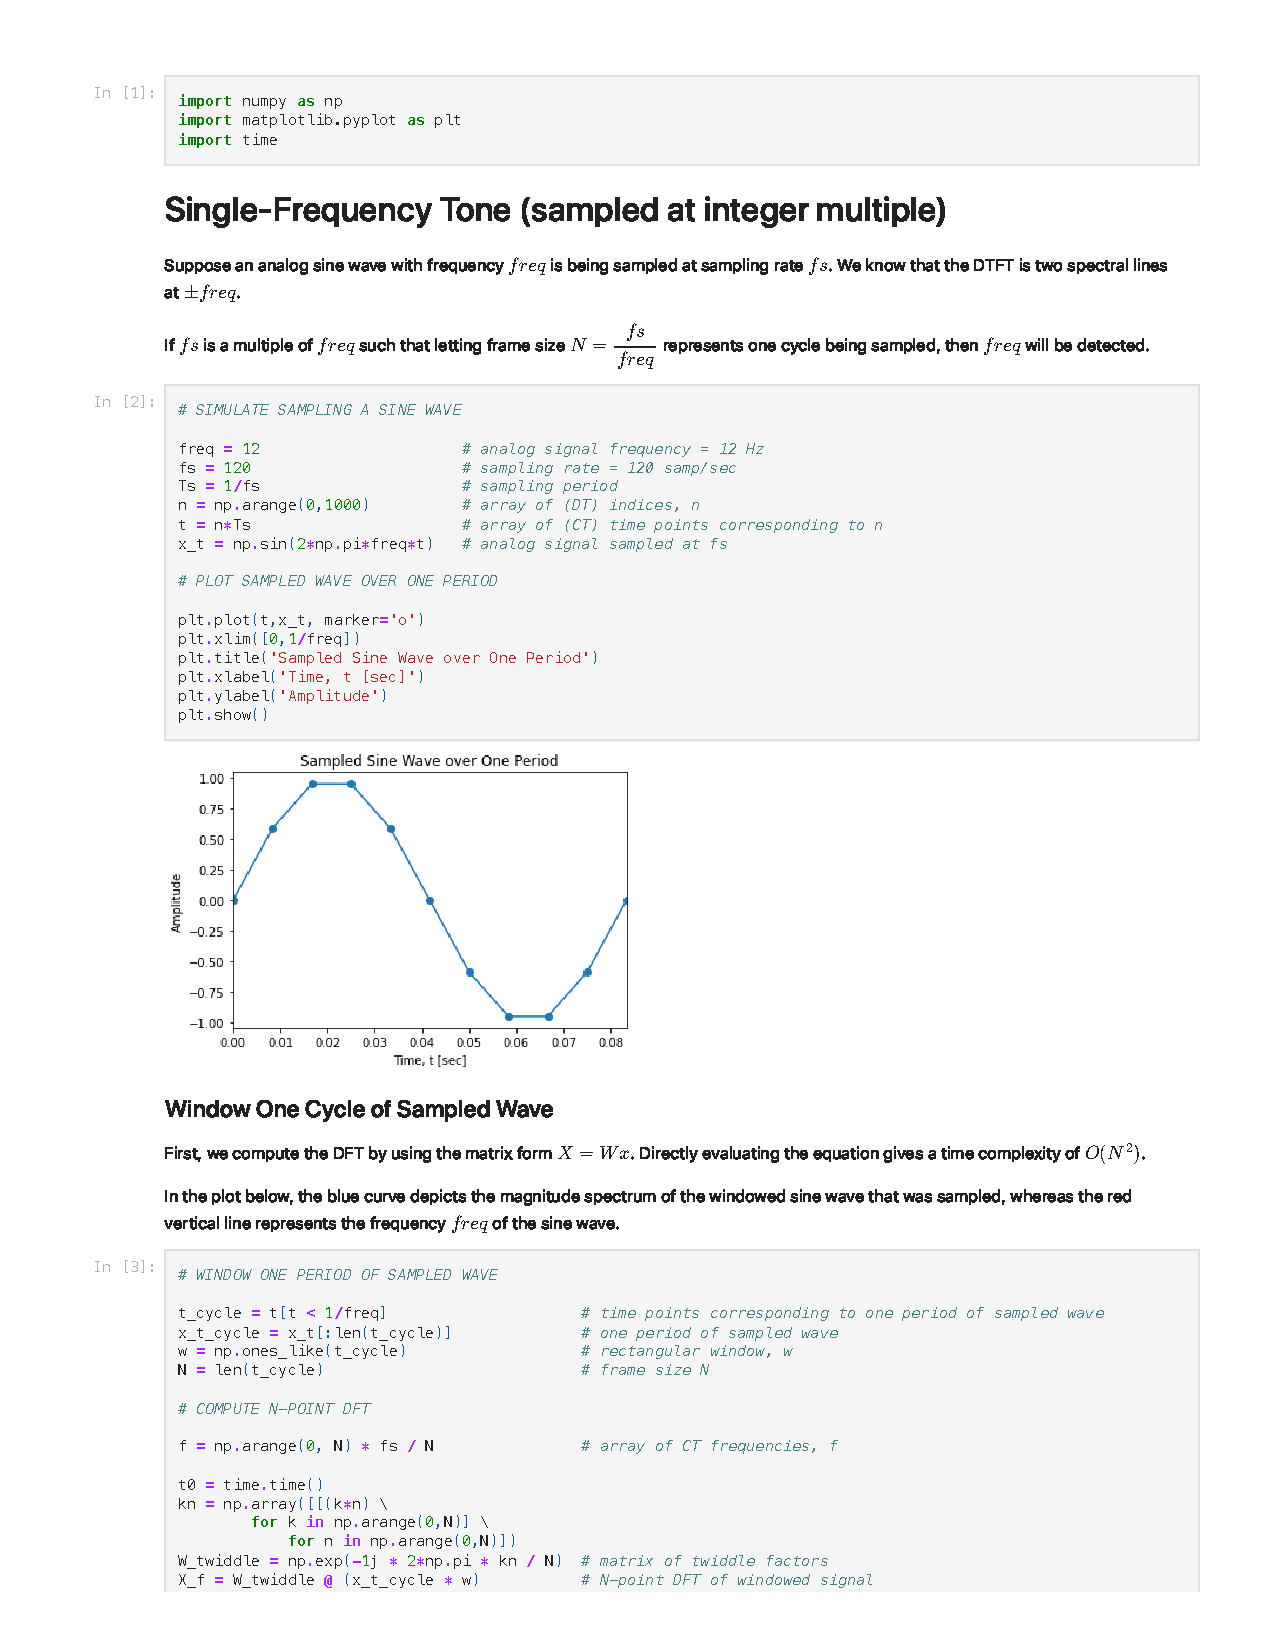
\includepdf[pages=-]{freq_analysis.pdf}

\end{document}